%!TEX TS-program = pdflatexmk

% Copyright (c) 2018 - 2022, Martin Scheidt (ISC license)
% Permission to use, copy, modify, and/or distribute this file for any purpose with or without fee is hereby granted, provided that the above copyright notice and this permission notice appear in all copies.

\documentclass[border=2]{standalone}

\usepackage[dev]{tikz-trackschematic}

\begin{document}
  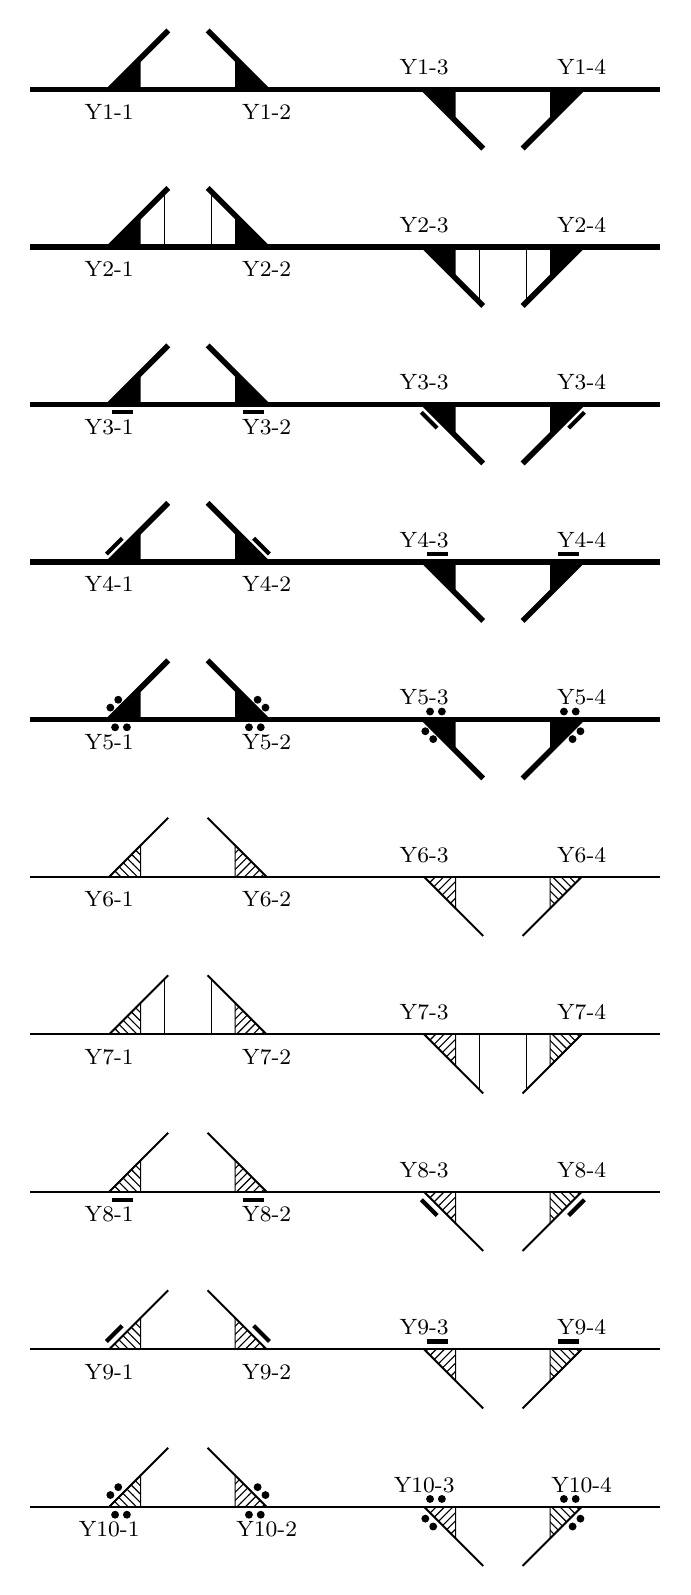
\begin{tikzpicture}
  
    \foreach \i in {1,2,...,10}{% base coordinate
      \coordinate (A\i) at ($(0,0) + 2*(0,-\i)$);
      \coordinate (B\i) at ($(8,0) + 2*(0,-\i)$);
    }

    \foreach \i in {1,2,...,5}{% draw main tracks on base coordinate
      \maintrack (A\i) --   (B\i);
    }

    \foreach \i in {6,7,...,10}{% draw secondary tracks on base coordinate
      \secondarytrack (A\i) --   (B\i);
    }

    \foreach \i in {1,2,...,10}{% coordinates for testing symbols
      \coordinate (Y\i-1) at ($(1,0) + 2*(0,-\i)$);
      \coordinate (Y\i-2) at ($(3,0) + 2*(0,-\i)$);
      \coordinate (Y\i-3) at ($(5,0) + 2*(0,-\i)$);
      \coordinate (Y\i-4) at ($(7,0) + 2*(0,-\i)$);
    }

    \foreach \i in {1,2,...,5}{% coordinates for testing symbols
      \maintrack  (Y\i-1) -- ++( 0.75, 0.75);
      \maintrack  (Y\i-2) -- ++(-0.75, 0.75);
      \maintrack  (Y\i-3) -- ++( 0.75,-0.75);
      \maintrack  (Y\i-4) -- ++(-0.75,-0.75);
    }

    \foreach \i in {6,7,...,10}{% coordinates for testing symbols
      \secondarytrack  (Y\i-1) -- ++( 0.75, 0.75);
      \secondarytrack  (Y\i-2) -- ++(-0.75, 0.75);
      \secondarytrack  (Y\i-3) -- ++( 0.75,-0.75);
      \secondarytrack  (Y\i-4) -- ++(-0.75,-0.75);
    }

    \turnout[forward ,branch=left ] at (Y1-1) label (Y1-1);
    \turnout[backward,branch=left ] at (Y1-2) label (Y1-2);
    \turnout[forward ,branch=right] at (Y1-3) label (Y1-3);
    \turnout[backward,branch=right] at (Y1-4) label (Y1-4);
    \turnout[forward ,branch=left ,fouling point] at (Y2-1) label (Y2-1);
    \turnout[backward,branch=left ,fouling point] at (Y2-2) label (Y2-2);
    \turnout[forward ,branch=right,fouling point] at (Y2-3) label (Y2-3);
    \turnout[backward,branch=right,fouling point] at (Y2-4) label (Y2-4);
    \turnout[forward ,branch=left ,points=right] at (Y3-1) label (Y3-1);
    \turnout[backward,branch=left ,points=right] at (Y3-2) label (Y3-2);
    \turnout[forward ,branch=right,points=right] at (Y3-3) label (Y3-3);
    \turnout[backward,branch=right,points=right] at (Y3-4) label (Y3-4);
    \turnout[forward ,branch=left ,points=left ] at (Y4-1) label (Y4-1);
    \turnout[backward,branch=left ,points=left ] at (Y4-2) label (Y4-2);
    \turnout[forward ,branch=right,points=left ] at (Y4-3) label (Y4-3);
    \turnout[backward,branch=right,points=left ] at (Y4-4) label (Y4-4);
    \turnout[forward ,branch=left ,points=moving] at (Y5-1) label (Y5-1);
    \turnout[backward,branch=left ,points=moving] at (Y5-2) label (Y5-2);
    \turnout[forward ,branch=right,points=moving] at (Y5-3) label (Y5-3);
    \turnout[backward,branch=right,points=moving] at (Y5-4) label (Y5-4);

    \turnout[forward ,branch=left ,operation=manual] at (Y6-1) label (Y6-1);
    \turnout[backward,branch=left ,operation=manual] at (Y6-2) label (Y6-2);
    \turnout[forward ,branch=right,operation=manual] at (Y6-3) label (Y6-3);
    \turnout[backward,branch=right,operation=manual] at (Y6-4) label (Y6-4);
    \turnout[forward ,branch=left ,operation=manual,fouling point] at (Y7-1) label (Y7-1);
    \turnout[backward,branch=left ,operation=manual,fouling point] at (Y7-2) label (Y7-2);
    \turnout[forward ,branch=right,operation=manual,fouling point] at (Y7-3) label (Y7-3);
    \turnout[backward,branch=right,operation=manual,fouling point] at (Y7-4) label (Y7-4);
    \turnout[forward ,branch=left ,operation=manual,points=right] at (Y8-1) label (Y8-1);
    \turnout[backward,branch=left ,operation=manual,points=right] at (Y8-2) label (Y8-2);
    \turnout[forward ,branch=right,operation=manual,points=right] at (Y8-3) label (Y8-3);
    \turnout[backward,branch=right,operation=manual,points=right] at (Y8-4) label (Y8-4);
    \turnout[forward ,branch=left ,operation=manual,points=left ] at (Y9-1) label (Y9-1);
    \turnout[backward,branch=left ,operation=manual,points=left ] at (Y9-2) label (Y9-2);
    \turnout[forward ,branch=right,operation=manual,points=left ] at (Y9-3) label (Y9-3);
    \turnout[backward,branch=right,operation=manual,points=left ] at (Y9-4) label (Y9-4);
    \turnout[forward ,branch=left ,operation=manual,points=moving] at (Y10-1) label (Y10-1);
    \turnout[backward,branch=left ,operation=manual,points=moving] at (Y10-2) label (Y10-2);
    \turnout[forward ,branch=right,operation=manual,points=moving] at (Y10-3) label (Y10-3);
    \turnout[backward,branch=right,operation=manual,points=moving] at (Y10-4) label (Y10-4);

  \end{tikzpicture}
\end{document}